% Presentation deck (EN) — the English counterpart of tese-pt/slides/.
% ~15 minutes. One slide, one idea. What is on the slide is what gets pointed at.
%
% ⚠️ THE DEFENCE IS IN PORTUGUESE, and this deck is not for it. It exists for the
% English-speaking audience of the paper: ICITS'27, Cusco, January 2027. The deck that
% gets presented at ISEP is tese-pt/slides/, and the two must not drift apart -- the
% figures and the numbers are the same, only the language changes.

\documentclass[aspectratio=169]{beamer}
\usetheme{Madrid}
\usecolortheme{seahorse}
\usepackage[T1]{fontenc}
\usepackage[english]{babel}
\usepackage{booktabs}
\usepackage{tikz}
\usetikzlibrary{positioning, arrows.meta, calc, decorations.pathreplacing}
\tikzset{every node/.append style={execute at begin node={\hyphenpenalty=10000\exhyphenpenalty=10000\relax}}}
% As figuras vem da arvore INGLESA, pela mesma razao pela qual o artigo as le de la: e
% a lingua deste documento. Sem um graphicspath valido o LaTeX compila em modo
% rascunho, o numero de paginas nao muda, e o PDF sai SEM AS IMAGENS -- um defeito que
% a contagem de paginas esconde.
\graphicspath{{../figures/}}
\usepackage{xcolor}
% A marca: o verde de `app/assets/logo.svg`, e o "G" e o trocadilho inteiro --
% inveSTIGATE + alliGATOR. Uma macro so, para o nome nunca sair escrito de duas
% maneiras diferentes em dois sitios.
\definecolor{marca}{HTML}{0A8F52}
\newcommand{\gator}{Investi\textcolor{marca}{G}ator}
\setbeamertemplate{navigation symbols}{}
\setbeamertemplate{caption}{\raggedright\insertcaption\par}

\title[\gator]{Explaining without predicting}
\titlegraphic{
\includegraphics[height=1.05cm]{logo_lockup.png}}
% The cover is the thesis title split at the colon: the evocative half here, the
% substantive one in the subtitle. Together they give the exact string that goes on the
% English inner cover, word for word.
\subtitle{\normalsize Anomaly detection and precedent retrieval for verifiable financial alerts}
\author[H.\ Santos]{Henrique José da Silva Santos \\
  \footnotesize Supervisor: Prof.\ Luís Gomes \quad Co-supervisor: Rafael Silva}
\institute[ISEP]{MEIA, Instituto Superior de Engenharia do Porto}
\date{\footnotesize}

\begin{document}

\begin{frame}\titlepage\end{frame}

% ══ 1. THE PROBLEM ══════════════════════════════════════════════════════════
\begin{frame}{Someone opens the app, sees this, and is left with three questions}
\begin{center}
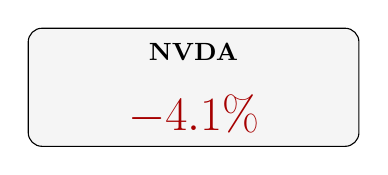
\begin{tikzpicture}
  \node[draw, rounded corners=5pt, minimum width=4.2cm, minimum height=1.5cm, fill=black!4] (t) {};
  \node[font=\small\bfseries] at ([yshift=4.5mm]t.center) {NVDA};
  \node[font=\LARGE\bfseries, text=red!65!black] at ([yshift=-3.5mm]t.center) {$-4.1\%$};
\end{tikzpicture}
\end{center}
\vspace{1mm}
\begin{enumerate}
  \item[\textbf{1.}] \textbf{Is this unusual?}\\
        \footnotesize 4\% is a lot for a quiet company. For another, it is a Tuesday.\\[2mm]
  \item[\textbf{2.}] \textbf{Was it the company, or the market?}\\
        \footnotesize If everything fell, the story is a different one.\\[2mm]
  \item[\textbf{3.}] \textbf{Has it happened before, and what followed?}\\
        \footnotesize Were there similar days? What did the price do afterwards?
\end{enumerate}
\vspace{2mm}
\begin{center}
\textbf{Current free applications answer none of them.}\\[1mm]
\footnotesize Recent products claim to go further. None shows the past cases, one by one,
with the measured outcome.
\end{center}
\end{frame}

\begin{frame}{What exists today}
\centering
\footnotesize
\begin{tabular}{lcccl}
\toprule
& \textbf{unusual?} & \textbf{company or market?} & \textbf{happened before?} & \textbf{cost} \\
\midrule
Broker application & --- & --- & --- & included \\
News aggregator & --- & --- & --- & free \\
Automated portfolio manager & --- & --- & --- & \% of portfolio \\
Professional terminal & \checkmark & \checkmark & \checkmark & not published \\
Generated summary (2025--26) & \multicolumn{3}{c}{\footnotesize \emph{claim to answer; do not show the evidence}} & free \\
\midrule
\textbf{This work} & \checkmark & \checkmark & \checkmark & \textbf{free} \\
\bottomrule
\end{tabular}
\vspace{5mm}

\begin{center}
Two recent products claim to answer the same question. Neither claims to \textbf{show the
evidence}: the past cases, one by one, with date and measured outcome.\\
\textbf{The difference I claim is not one of fluency: it is one of verifiability.}
\end{center}
\end{frame}

% ══ 2. THE SYSTEM ═══════════════════════════════════════════════════════════
\begin{frame}{What the system does}
\begin{center}
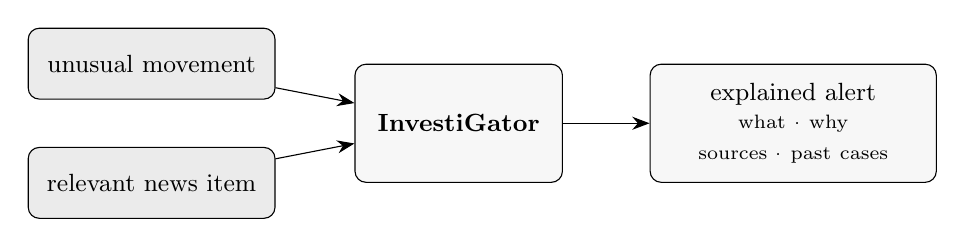
\begin{tikzpicture}[
  font=\small, >={Stealth[length=2.2mm]},
  gat/.style={draw, rounded corners, fill=black!8, align=center, text width=2.9cm, minimum height=0.9cm},
  sis/.style={draw, rounded corners, fill=black!3, align=center, text width=2.4cm, minimum height=1.5cm},
  sa/.style={draw, rounded corners, fill=black!3, align=center, text width=3.4cm, minimum height=1.5cm},
]
  \node[gat] (g1) {unusual movement};
  \node[gat, below=6mm of g1] (g2) {relevant news item};
  \node[sis] (s) at ($(g1)!0.5!(g2) + (3.9,0)$) {\textbf{InvestiGator}};
  \node[sa, right=1.1cm of s] (o) {explained alert\\[2pt]
    \scriptsize what · why\\ \scriptsize sources · past cases};
  \draw[->] (g1) -- (s); \draw[->] (g2) -- (s); \draw[->] (s) -- (o);
\end{tikzpicture}
\end{center}
\vspace{4mm}
\begin{center}
\large And there is one thing it \textbf{refuses} to do.
\end{center}
\end{frame}

\begin{frame}{It does not forecast prices}
\begin{center}
\Large
It never says the price will rise.\\[2mm]
It never says to buy.\\[2mm]
It never shows a price target.
\end{center}
\vspace{6mm}
\begin{center}
\normalsize
It looks like a limitation. It is the opposite:\\
\textbf{it is what makes everything else verifiable.}\\[2mm]
\footnotesize A statement about what already happened is checked against the record.\\
A forecast cannot be checked when it is read.
\end{center}
\end{frame}

% ══ 3. THE FOUR TECHNIQUES ══════════════════════════════════════════════════
\begin{frame}{Technique 1: is it unusual?}
Compare today with \textbf{the 20 previous days of the same stock}.
\begin{center}
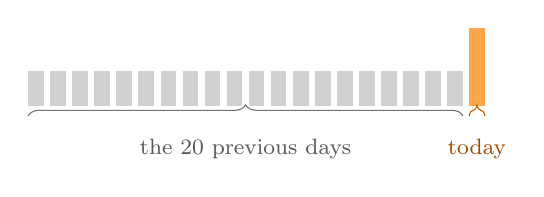
\begin{tikzpicture}[font=\footnotesize]
  \foreach \i in {0,...,19} { \fill[black!18] (\i*0.28,0) rectangle (\i*0.28+0.2,0.45); }
  \fill[orange!70] (20*0.28,0) rectangle (20*0.28+0.2,1.0);
  \draw[decorate, decoration={brace, amplitude=4pt}, black!55] (0,-0.12) -- (19*0.28+0.2,-0.12)
    node[midway, below=5pt, black!65] {the 20 previous days};
  \draw[decorate, decoration={brace, amplitude=4pt}, orange!75!black]
    (20*0.28,-0.12) -- (20*0.28+0.2,-0.12) node[midway, below=5pt, text=orange!60!black] {today};
\end{tikzpicture}
\end{center}
\vspace{1mm}
\begin{center}
$z = \dfrac{\text{today's move} - \text{mean}}{\text{standard deviation}}$
\end{center}
\vspace{2mm}
\footnotesize
$z=+7$ means the same thing for a quiet company and for a volatile one.\\
\textbf{The day being judged is excluded from the norm it is judged against.} Without that, it would be cheating.
\end{frame}

\begin{frame}{Technique 2: was it the company, or the market?}
A $+6.29\%$ can be the company or it can be the market. The broker application
shows \textbf{the same number} in both cases.
\vspace{2mm}
\begin{center}
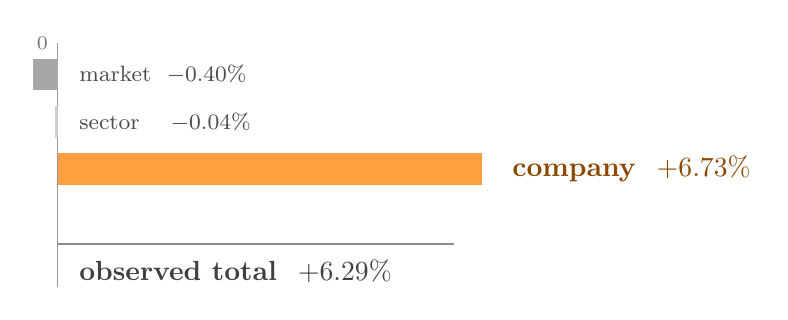
\begin{tikzpicture}[font=\footnotesize]
  % AMD, dia real: +6.29% = -0.40 mercado -0.04 setor +6.73 empresa
  \draw[black!40] (0,0) -- (0,3.1);
  \node[black!55, font=\scriptsize, left] at (0,3.1) {0};
  \fill[black!35]      (0,2.5) rectangle (-0.40*0.8,2.9);
  \fill[black!20]      (0,1.9) rectangle (-0.04*0.8,2.3);
  \fill[orange!75]     (0,1.3) rectangle (6.73*0.8,1.7);
  \node[right, black!70] at (0.15,2.7) {market \ $-0.40\%$};
  \node[right, black!70] at (0.15,2.1) {sector \ \ \ $-0.04\%$};
  \node[right=5.5cm, text=orange!55!black, font=\bfseries] at (0.15,1.5) {company \ $+6.73\%$};
  \draw[black!45, thick] (0,0.55) -- (6.29*0.8,0.55);
  \node[right, black!75, font=\bfseries] at (0.15,0.2) {observed total \ $+6.29\%$};
\end{tikzpicture}
\end{center}
\vspace{1mm}
\footnotesize
AMD rose \textbf{despite} the market and the sector pulling the other way.
The \emph{betas} are estimated \textbf{from previous days only}.\\
\textbf{Caveat:} the parts always add up, because the company's is the residual, and that does
not prove they are well estimated. Median $R^2$ of $0.460$, and negative in one case.\\
\textbf{It is the only one of the four without a research question:} there is no correct answer
to compare against, so what is measured is the fit, not the accuracy.
\end{frame}

\begin{frame}{Technique 3: has it happened before?}
Searching by words fails in \textbf{both} directions:
\vspace{2mm}
\begin{center}
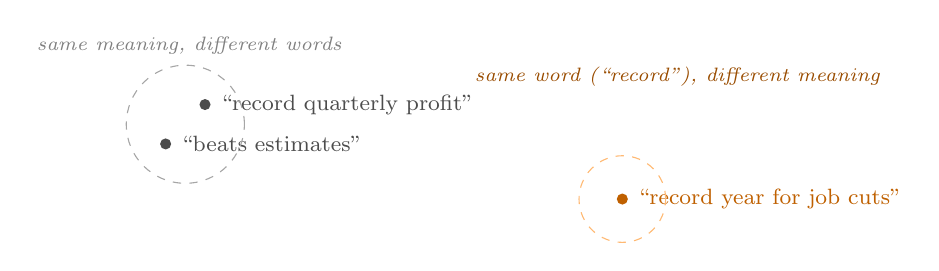
\begin{tikzpicture}[font=\footnotesize]
  \fill[black!70] (0.6,1.5) circle (2pt) node[right=2pt] {``beats estimates''};
  \fill[black!70] (1.1,2.0) circle (2pt) node[right=2pt] {``record quarterly profit''};
  \draw[black!35, dashed] (0.85,1.75) circle (0.75);
  \node[black!50, font=\scriptsize\itshape] at (0.9,2.75) {same meaning, different words};
  \fill[orange!75!black] (6.4,0.8) circle (2pt) node[right=2pt] {``record year for job cuts''};
  \draw[orange!55, dashed] (6.4,0.8) circle (0.55);
  \node[orange!60!black, font=\scriptsize\itshape] at (7.1,2.35) {same word (``record''), different meaning};
\end{tikzpicture}
\end{center}
\vspace{1mm}
Each headline becomes \textbf{384 numbers}: a coordinate of meaning.\\
They are compared by the \textbf{angle} between them.
\vspace{2mm}

Then, for each past case, what the price did at $+1$, $+3$ and $+5$ days is measured.\\
\footnotesize \textbf{It is a measurement of the past, not a forecast.}
\end{frame}

\begin{frame}{Technique 4: is it worth interrupting?}
Here there is no obvious formula. This is the place to \textbf{learn from the data}.
\vspace{3mm}
\begin{itemize}
  \item \textbf{79\,753} examples built from news and prices (2018--2023)
  \item The question: \emph{after this headline, was there an abnormally large move?}
        \textbf{In absolute value}, never in which direction
\end{itemize}
\vspace{1mm}

% ⚠️ ESTE BLOCO SUBSTITUI UM BULLET QUE DIZIA "divisão cronológica com embargo" E MAIS NADA.
% É a pergunta de credibilidade de qualquer tese com um modelo treinado ("como sabes que ele não
% viu o futuro?") e a resposta era uma linha de texto, ou seja uma afirmação. Passa a ser
% mostrada: a divisão vê-se, e o teste que a impõe está escrito ao lado. Não custa um frame
% novo, porque ocupa o espaço dos bullets que substitui.
\centering

\begin{tikzpicture}[font=\scriptsize]
  \fill[black!55] (0,0) rectangle (6.3,0.52);
  \fill[orange!45] (6.3,0) rectangle (6.72,0.52);
  \fill[black!30] (6.72,0) rectangle (8.12,0.52);
  \fill[orange!45] (8.12,0) rectangle (8.54,0.52);
  \fill[black!55] (8.54,0) rectangle (9.94,0.52);
  \node[white, font=\scriptsize\bfseries] at (3.15,0.26) {TRAIN};
  \node[white, font=\scriptsize\bfseries] at (7.42,0.26) {VALID.};
  \node[white, font=\scriptsize\bfseries] at (9.24,0.26) {TEST};
  % Os dois rótulos dizem a MESMA coisa de propósito: um a dizer "embargo" e o outro a dizer
  % "5 dias" lia-se como duas bandas diferentes, quando são a mesma regra aplicada duas vezes.
  \node[orange!60!black, anchor=south, font=\tiny] at (6.51,0.60) {embargo};
  \node[orange!60!black, anchor=south, font=\tiny] at (8.33,0.60) {embargo};
  \draw[->, black!45] (0,-0.22) -- (9.94,-0.22) node[right, black!60, font=\tiny] {time};
\end{tikzpicture}
\vspace{3mm}

\raggedright\footnotesize
Split by \textbf{whole days} with a \textbf{five-day} embargo, never by rows: two headlines
from the same day cannot fall on opposite sides. And the guarantee is not promised, it is
\textbf{enforced by a test}: two absurd futures ($+300\%$ and $-99\%$) over the same past must
produce \textbf{identical} inputs and \textbf{different} labels. If the future leaked, the inputs
would change.
\end{frame}

% ══ 4. ONE REAL ALERT ═══════════════════════════════════════════════════════
\begin{frame}{One real alert, from start to finish}
\footnotesize Meta, 12 July 2026. \emph{``Mark Zuckerberg Said Meta's AI Bets `Haven't Come
to Fruition Yet' as Shares Fell 5\%''}
\vspace{2mm}
\centering
\scriptsize
\begin{tabular}{rll}
\toprule
& \textbf{stage} & \textbf{what happened} \\
\midrule
2 & names the company? & ``Meta'', ``Zuckerberg'' \checkmark \\
3 & is it recent? & less than 2 days \checkmark \\
4 & similar cases & MSFT $0.46$ · NVDA $0.51$ · NVDA $0.46$ \\
5 & evidence strong enough? & best $0.51 \ge 0.45$ \checkmark \\
6 & worth interrupting? & $54\% \ge 50\%$ \checkmark \\
9 & sent & to the channel, and stored \\
\bottomrule
\end{tabular}
\vspace{3mm}

\begin{center}
\footnotesize The outcomes went \textbf{in opposite directions}: $+2.70\%$ · $-3.87\%$ · $+5.05\%$\\
That is why they are shown \textbf{one by one}: an average would hide it.
\end{center}
\end{frame}

% ══ 5. RESULTS ═════════════════════════════════════════════════════════════
\begin{frame}{Result 1: detection \textcolor{green!50!black}{\textbf{yes}}}
A good detector should fire at a \textbf{similar} rate across different companies.
\vspace{2mm}
\centering
\begin{tabular}{lccc}
\toprule
& \textbf{min} & \textbf{max} & \textbf{spread} \\
\midrule
\emph{z}-score & $0.016$ & $0.031$ & $\mathbf{0.015}$ \\
Fixed threshold of 3\% & $0.009$ & $0.353$ & $0.344$ \\
\bottomrule
\end{tabular}
\vspace{4mm}

\begin{center}
More than \textbf{20 times} more consistent.\\[2mm]
\small And it also beats two learned methods:
$F_1$ of $\mathbf{0.530}$ against $0.269$ and $0.280$.
\end{center}
\end{frame}

\begin{frame}{Result 2: precedents \textcolor{green!50!black}{\textbf{yes}}}
\centering
\begin{tabular}{lc}
\toprule
\textbf{method} & \textbf{precision@5} \\
\midrule
\textbf{By meaning (the method)} & $\mathbf{0.514}$ \\
Always the largest sector & $0.467$ \\
By shared words & $0.346$ \\
At random (the floor) & $0.240$ \\
The most recent & $0.126$ \\
\bottomrule
\end{tabular}
\vspace{2mm}

\begin{itemize}
  \small
  \item Half the corpus is technology: \textbf{always returning technology} is worth $0.467$
        with no model at all. The real margin is $+0.047$, not $+0.274$.
  \item \textbf{But that alternative is right about everything in one sector and nothing in the
        other four.} Within each sector the method wins in all \textbf{five}: $0.448$ in energy,
        against a floor of $0.072$.
  \item On the full corpus, under the causal constraint of production: \textbf{0.513}, with a
        floor of \textbf{0.259} and a margin of \textbf{$+0.254$}. The \textbf{0.595} is the
        symmetric test of scale.
  \item And it \textbf{captures theme, not direction}, which is why the cases appear one by one.
\end{itemize}
\end{frame}

\begin{frame}{Result 3: triage \textcolor{red!60!black}{\textbf{no}}}
\centering
\begin{tabular}{lc}
\toprule
\textbf{model} & \textbf{PR-AUC} \\
\midrule
\textbf{Volatility only} & $\mathbf{0.542}$ \\
Context only & $0.538$ \\
Context + text & $0.496$ \\
Text only & $0.439$ \\
\bottomrule
\end{tabular}
\vspace{3mm}

\begin{center}
\textbf{No model that reads the text beats volatility.}
\end{center}
\vspace{2mm}
\footnotesize
It was the opposite of what I expected. I checked it three ways:
a re-test under conditions favourable to the text ($0.533$, still below),
resampling by groups, and \textbf{nine} different definitions of the label: volatility wins
in all nine.
\end{frame}

\begin{frame}{The mistake I found in my own work}
I had written that triage \emph{``almost quadruples''} precision: from $0.163$ to $0.632$.
\vspace{3mm}

The $0.163$ came from the ``always alert'' model, which gives everything the same score.\\
\textbf{With everything tied, the metric breaks ties by file order}, and the file is sorted by
date and by company name.
\vspace{3mm}
\begin{center}
\large That number was not measuring choosing blindly.\\
\textbf{It was measuring choosing alphabetically.}
\end{center}
\vspace{3mm}
\footnotesize
Real chance gives $0.379$ $\Rightarrow$ the gain is \textbf{1.67$\times$}, not almost four.\\
And a table of \textbf{13 constants} gives $0.662$: it beats the trained model.
\end{frame}

\begin{frame}{And I found it again, one level up}
\small
The system decided whether to alert with a \textbf{fixed threshold} on the model's score: anything
above $0.50$ passes.
\vspace{-1mm}
\begin{center}
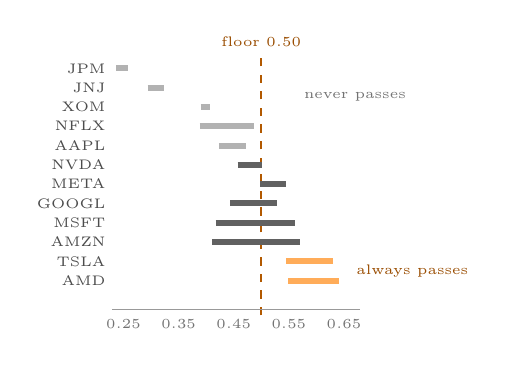
\begin{tikzpicture}[font=\tiny, x=7.0cm, y=0.245cm]
  \draw[dashed, thick, orange!70!black] (0.50,-0.8) -- (0.50,12.6)
    node[above, text=orange!60!black] {floor $0.50$};
    % Variaveis do \foreach nunca podem chamar-se \c \t \l \i \o: sao comandos do
  % LaTeX (cedilha, til, l barrado, i sem ponto, o barrado) e o \foreach substitui-os
  % tambem DENTRO das palavras. Ver a Figura 6.1, onde \c transformava "avaliacao"
  % em "avalia<custo>cao" sem um unico aviso de compilacao.
  \foreach \xn/\xtk/\xa/\xb/\xcor in {
    12/JPM/0.237/0.258/black!30, 11/JNJ/0.294/0.324/black!30,
    10/XOM/0.390/0.407/black!30, 9/NFLX/0.388/0.486/black!30,
    8/AAPL/0.423/0.472/black!30, 7/NVDA/0.457/0.501/black!62,
    6/META/0.498/0.545/black!62, 5/GOOGL/0.444/0.528/black!62,
    4/MSFT/0.417/0.561/black!62, 3/AMZN/0.411/0.571/black!62,
    2/TSLA/0.545/0.630/orange!65, 1/AMD/0.549/0.641/orange!65}
  { \node[left, black!70] at (0.235,\xn) {\xtk};
    \draw[line width=2.2pt, color=\xcor] (\xa,\xn) -- (\xb,\xn); }
  \node[right, text=black!55] at (0.56,10.5) {never passes};
  \node[right, text=orange!60!black] at (0.655,1.5) {always passes};
  \draw[black!40] (0.23,-0.5) -- (0.68,-0.5);
  \foreach \x in {0.25,0.35,0.45,0.55,0.65}
    \node[below, black!55] at (\x,-0.5) {$\x$};
\end{tikzpicture}
\end{center}
\vspace{-1mm}
\begin{center}
In \textbf{48\%} of the distinct headlines, the outcome was determined\\
by the \textbf{company} before the headline was read.
\end{center}
\vspace{1mm}
{\footnotesize In no logged assessment did Apple reach the floor, with a maximum of $0.472$; AMD exceeded it in all of them. Counted per decision the fraction rises to $60\%$, inflated by the minute-by-minute re-scoring.}
\end{frame}

\begin{frame}{And the obvious fix was wrong too}
\textbf{The temptation:} if a fixed threshold measures the company and not the news item, make it
\emph{relative to each company}, which is exactly what the \emph{z}-score did for prices.
\vspace{3mm}

I simulated it \textbf{before} writing any code. Half of it is solved: all twelve become
represented.
\vspace{2mm}

\textbf{But} in companies whose score is nearly constant the percentile falls \emph{on top of} the
constant and almost everything ties above it. JNJ would pass \textbf{874} times.
\vspace{3mm}
\begin{center}
\large A defect is not fixed by introducing the neighbouring one.
\end{center}
\vspace{3mm}
\footnotesize
\textbf{What was done:} the model stopped deciding and started \textbf{ranking}, under a budget of
5 alerts per day. And that closed a divergence: the dissertation \emph{evaluated} a budget policy
while the system \emph{deployed} a threshold one.
\end{frame}

% ══ 6. WHAT I LEARNED ══════════════════════════════════════════════════════
\begin{frame}{So what is the model worth? Two measurements that answer}
\small
\begin{columns}[T]
\begin{column}{0.47\textwidth}
\textbf{1. I took the news away.}\\[1mm]
{\scriptsize A \emph{lookup table}: one fixed number per company, zero information about the
headline.}
\vspace{1mm}
\begin{center}\scriptsize
\begin{tabular}{lc}
\toprule
\textbf{what it sees} & \textbf{PR-AUC} \\
\midrule
the deployed one, nine inputs & $0.538$ \\
\textbf{the company only} & $\mathbf{0.534}$ \\
nothing about the company & $0.378$ \\
headline length only & $0.378$ \\
\bottomrule
\end{tabular}
\end{center}
\vspace{1mm}
{\scriptsize A difference of $0.004$, and $0.378$ is the floor. \textbf{The deployed model is a
lookup table.}}
\end{column}
\begin{column}{0.47\textwidth}
\textbf{2. I compared the whole system.}\\[1mm]
{\scriptsize Precision over the five news items the product shows per day.}
\vspace{1mm}
\begin{center}\scriptsize
\begin{tabular}{lc}
\toprule
\textbf{policy} & \textbf{prec.@5} \\
\midrule
at random & $0.375$ \\
whoever moved most today & $0.489$ \\
\textbf{the system} & $\mathbf{0.632}$ \\
volatility, thirteen constants & $0.662$ \\
oracle & $0.968$ \\
\bottomrule
\end{tabular}
\end{center}
\vspace{1mm}
{\scriptsize It beats the realistic alternative. \textbf{But the oracle is the new information:}
the important news \emph{is} in the batch.}
\end{column}
\end{columns}
\vspace{2mm}
\begin{center}
The missing margin is not in better data. It is in \textbf{separating two news items from the
same company on the same day}.
\end{center}
\end{frame}

\begin{frame}{``And where is the artificial intelligence engineering?''}
\small
I start with the uncomfortable part: this work trains \textbf{one} model, and it is a logistic
regression with nine inputs that \textbf{lost} to a single-variable baseline.
\vspace{2mm}

\begin{center}
\textbf{The engineering is not in the size of the model.}\\
It is in what had to be built so that that number, and the negative conclusion
it supports, can be \emph{trusted}.
\end{center}
\vspace{2mm}

\begin{columns}[T]
\begin{column}{0.48\textwidth}
{\footnotesize
\textbf{1.} The dataset is \textbf{built}, not found: $79\,753$ rows that did not exist.
\\[1mm]
\textbf{2.} The label is a \textbf{decision}, which is why \textbf{nine} alternative definitions
were measured.\\[1mm]
\textbf{3.} The temporal separation is enforced by a \textbf{test} that mutates the future,
not promised.\\[1mm]
\textbf{4.} The probabilities are calibrated, and their bias is \textbf{measured}.
}
\end{column}
\begin{column}{0.48\textwidth}
{\footnotesize
\textbf{5.} The model, the calibrator and the run are \textbf{versioned}.\\[1mm]
\textbf{6.} The deployed model \textbf{is} the evaluated model: exported to a lightweight
format, with the fidelity of the conversion measured rather than assumed.\\[1mm]
\textbf{7.} What runs is \textbf{observed}: every decision is logged and confronted days later
with what the price did. That is how it became known that it was \emph{not} helping.
}
\end{column}
\end{columns}
% 2mm punha a caixa 0.52pt acima do slide. Meio ponto nao se ve, mas o padrao dos materiais
% deste projecto e zero overfull, e um aviso tolerado e um aviso que se deixa de ler.
\vspace{0.5mm}

\begin{center}
\footnotesize The hard part was not choosing the technique. It was building the evaluation that
\textbf{can say no}, and then believing it.
\end{center}
\end{frame}

\begin{frame}{Limitations, said before being asked, and what closes them}
\textbf{Every limitation was measured}, and the right-hand column is the work it asks for.
\vspace{1.5mm}
\begin{center}
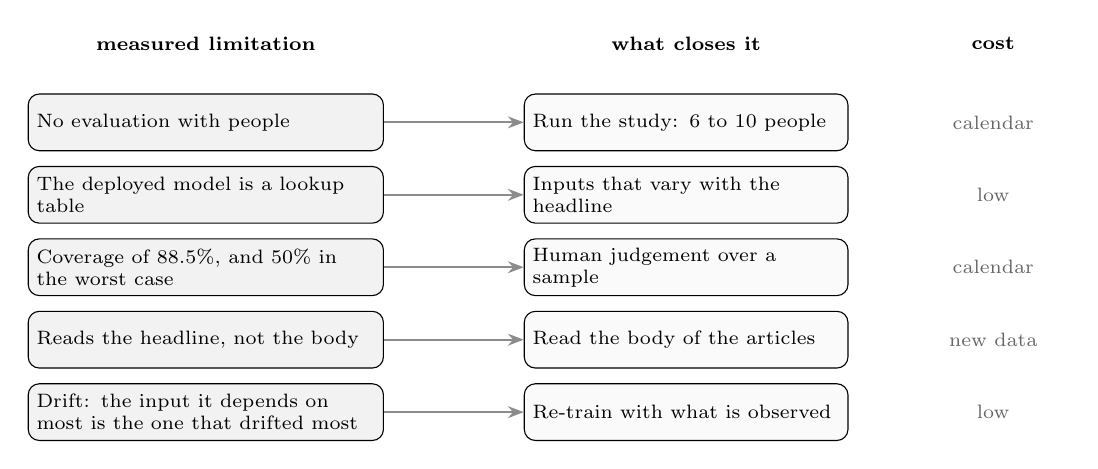
\begin{tikzpicture}[font=\scriptsize, >={Stealth[length=2mm]},
  lim/.style={draw, rounded corners, align=left, text width=4.3cm, inner sep=3pt,
              minimum height=0.72cm, fill=black!5},
  fut/.style={draw, rounded corners, align=left, text width=3.9cm, inner sep=3pt,
              minimum height=0.72cm, fill=black!2},
  cst/.style={align=center, text width=1.7cm, text=black!60},
]
  \node[font=\bfseries\scriptsize] at (0,1.0)   {measured limitation};
  \node[font=\bfseries\scriptsize] at (6.1,1.0) {what closes it};
  \node[font=\bfseries\scriptsize] at (10.0,1.0) {cost};
  % ATENCAO: nunca usar \c \l \i \t \o como variaveis do \foreach (sao comandos do LaTeX)
  \foreach \xn/\xlim/\xfut/\xcus in {%
    0/{No evaluation with people}/{Run the study: 6 to 10 people}/{calendar},%
    1/{The deployed model is a lookup table}/{Inputs that vary with the headline}/{low},%
    2/{Coverage of $88.5\%$, and $50\%$ in the worst case}/{Human judgement over a sample}/{calendar},%
    3/{Reads the headline, not the body}/{Read the body of the articles}/{new data},%
    4/{Drift: the input it depends on most is the one that drifted most}/{Re-train with what is observed}/{low}%
  } {
    \node[lim] (L\xn) at (0,-\xn*0.92) {\xlim};
    \node[fut] (F\xn) at (6.1,-\xn*0.92) {\xfut};
    \node[cst] at (10.0,-\xn*0.92) {\xcus};
    \draw[->, thick, black!45] (L\xn) -- (F\xn);
  }
\end{tikzpicture}
\end{center}
\vspace{0.5mm}
{\footnotesize \textbf{Two more:} the delay is the \emph{source}'s and not the infrastructure's
($\approx$353\,min to detect, 5\,s to deliver); and \textbf{nothing is ever re-trained}, because the
case base grows on its own and the weights do not.}
\end{frame}

% Closes the loop of the first frame: the three questions the deck opened with, answered on
% the screen of a REAL case, captured from production. The day was not picked for looking good.
\begin{frame}{The three questions, answered on screen}
\begin{columns}[T]
\begin{column}{0.62\textwidth}
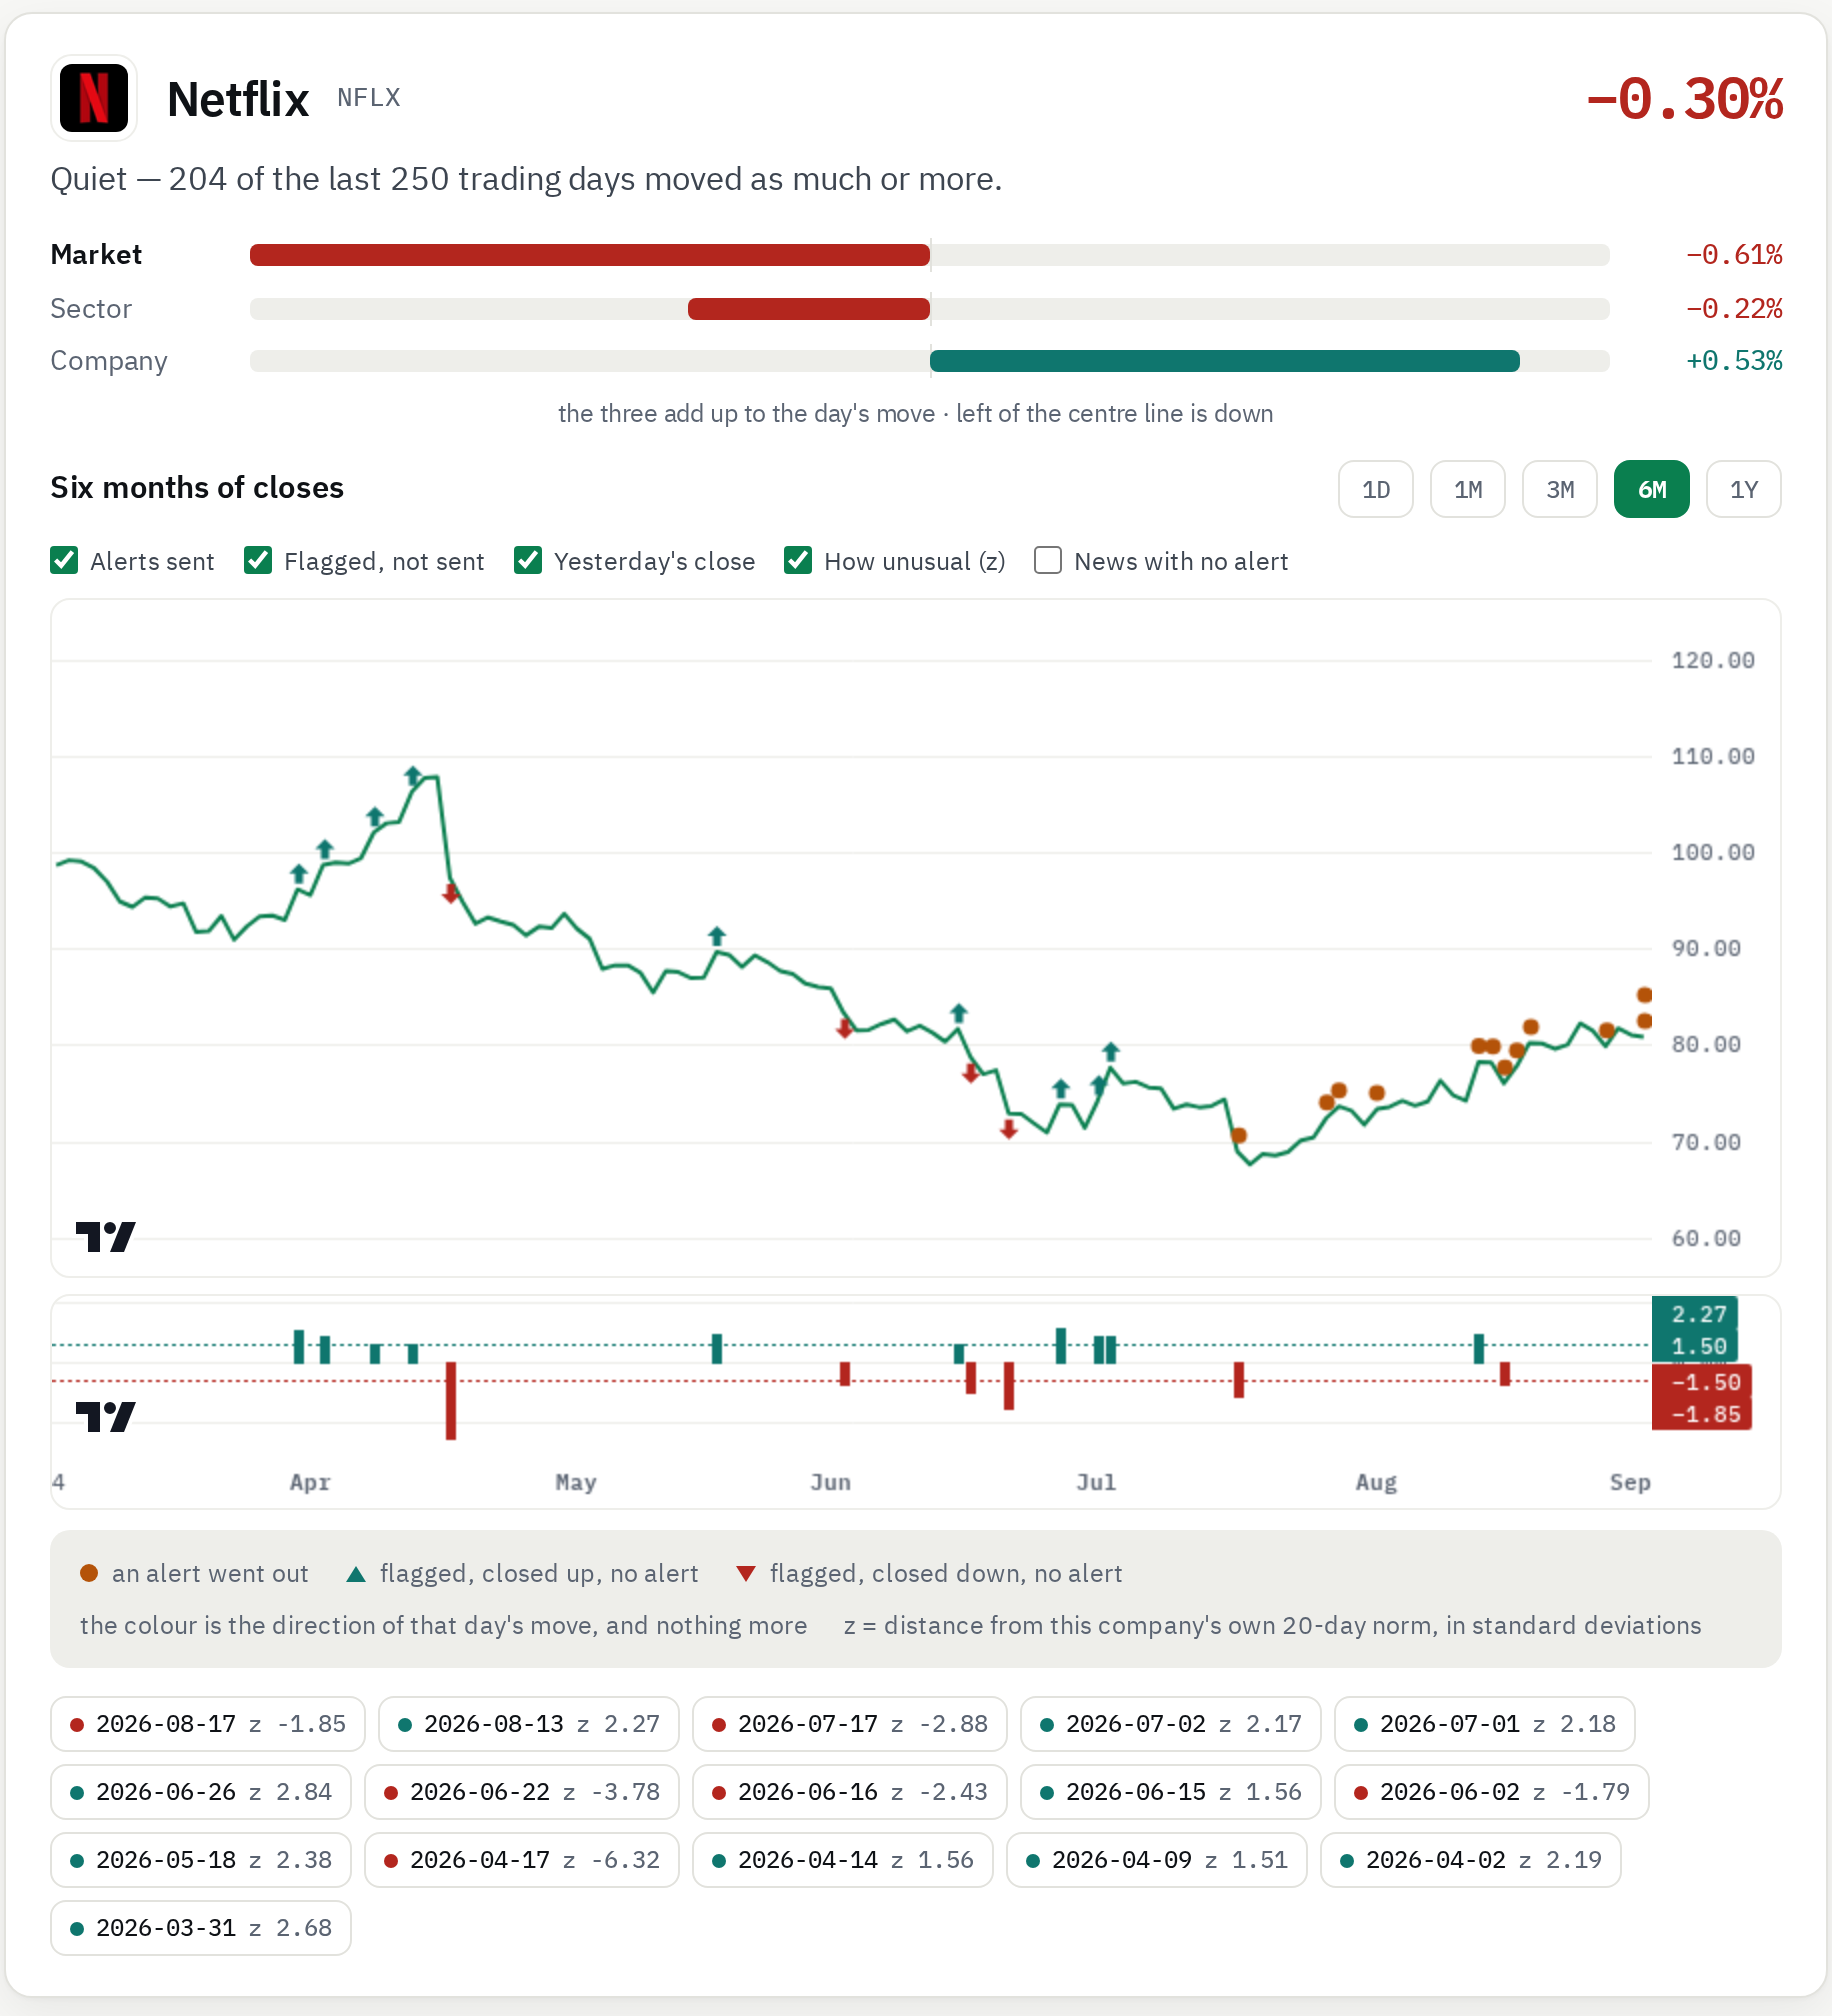
\includegraphics[height=0.68\textheight]{app_v7_empresa.png}
\end{column}
\begin{column}{0.35\textwidth}
\small
\textbf{1. Is it unusual?}\\
{\footnotesize In words, before the number: $204$ of the last $250$ days moved
this much or more. The verdict is \emph{``Quiet''}, and it comes before any value.}
\vspace{3mm}

\textbf{2. Was it the company?}\\
{\footnotesize \textbf{No.} The stock falls $0.30\%$, but the company's own
contribution is \textbf{positive} ($+0.53\%$): what pulls it down is the
\textbf{market} ($-0.61\%$). The percentage alone sent the reader looking
inside the company for a reason that was outside it.}
\vspace{3mm}

\textbf{3. Has it happened before?}\\
{\footnotesize The days marked on the curve, and the precedents inside the text of the alert.}
\end{column}
\end{columns}
\end{frame}

% ══ 7. DEMONSTRATION ═══════════════════════════════════════════════════════
\begin{frame}{Demonstration}
\begin{center}
{\large The system is live.} \quad \textbf{[recording]}\\[2mm]
{\footnotesize a real news item, from the moment it arrives to the alert that goes out}
\end{center}
\vspace{1mm}
\begin{center}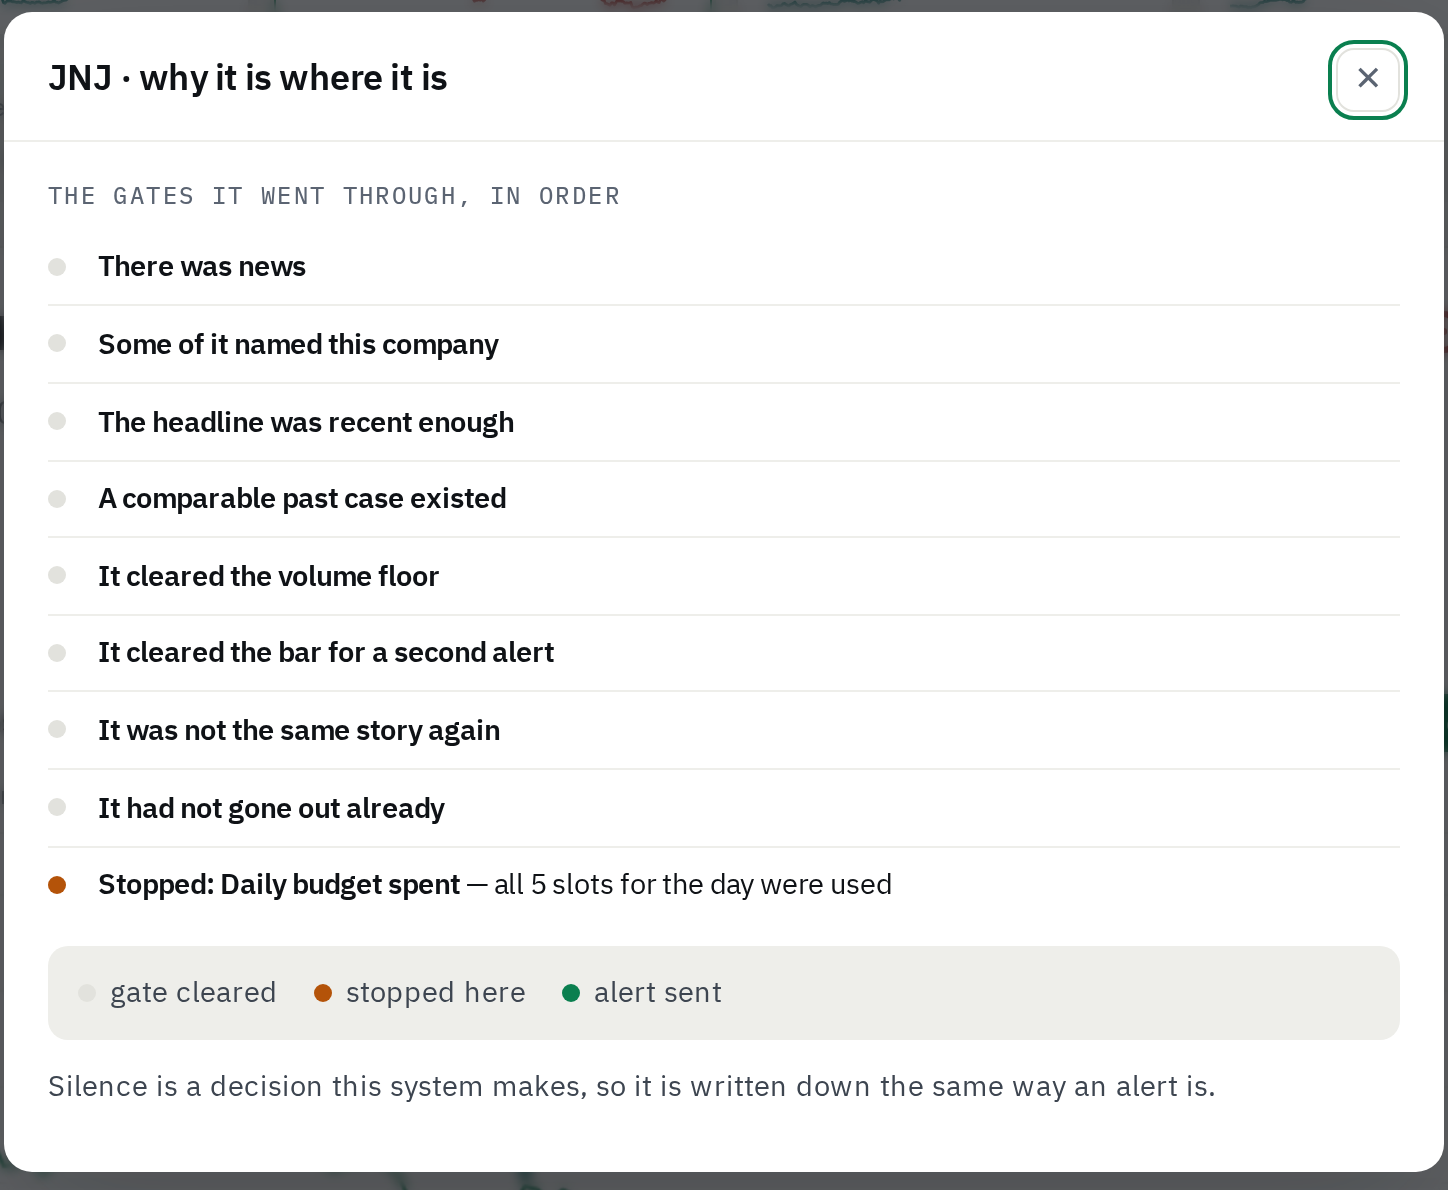
\includegraphics[width=0.97\textwidth,height=0.46\textheight,keepaspectratio]{app_v7_silencio.png}\end{center}

{\footnotesize The path of one candidate through the gates, to where it stopped. \textbf{It is the
part a live demonstration cannot show}: nine out of ten scans send nothing, and the silence
is written down like an alert.}
% ⚠️ This deck is NOT the one presented at the defence -- that one is tese-pt/slides/.
%    Here the image stands on its own: for a conference talk there is no live system to
%    show, and the funnel capture is what carries the point.
\end{frame}

% What I learned lives here, and not in a frame of its own: it stays on screen during the
% questions, which is a better place than a slide that goes by in a glance.
\begin{frame}[plain]{What I learned}
\begin{enumerate}
  \item \textbf{The baseline matters as much as the model.}\\
        \footnotesize The most useful result of the work came from looking at what I was
        comparing against.\\[2mm]
  \item \textbf{Where a model is placed matters as much as the model.}\\
        \footnotesize Mine worked on its own and stopped being useful behind two simple filters
        that were already doing the work.\\[2mm]
  \item \textbf{The simpler technique won three times.}\\
        \footnotesize Against Isolation Forest and against the model that reads the text, which are
        \emph{simple against complex}. And a table of constants beat the deployed model, which
        is a different case: there the model was interpretable, and lost for \textbf{lack of
        information}.
\end{enumerate}
\vspace{4mm}
\begin{center}
\small The hard part was not choosing the most advanced technique.\\
It was building the evaluation \textbf{able to say that it was not needed}.\\[6mm]
{\Large \textbf{Thank you.}\quad Questions?}
\end{center}
\end{frame}

\end{document}
